\section{Considerations on Grain-Matrix Interfaces}\label{sec:grain_matrix}

\begin{figure}
    \begin{center}
        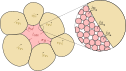
\includegraphics[width=0.95\textwidth]{img/model_development/grain_matrix_overview}
    \end{center}
    \caption{Principle of the Multiscale Approach with Coarse Particle Skeleton and Fine Particle Matrix Continuum}\label{fig:model_development/grain_matrix_overview}
\end{figure}

Since the investigated material is characterized by particle sizes in several orders of magnitude (fine alumina with $\Diameter \approx \qty{20}{\micro\meter}$ and aggregates with $\Diameter \approx \qty{2}{\milli\meter}$), direct simulation of contact between all possible occuring particles is not possible.
A fine discretization on all particles would lead to excessive high count of nodes on the coarse particles.
A coarse discretization on all particles would lead to a degenerated shape of the small ones.
A fine discretization on small ones and a coarse on large ones, however, would lead to large numerical errors in contacts due to heavily different discretization widths on both sides.
Therefore, another approach has to be taken.

In the following, a multiscale approach consisting of a finely powdered continuum matrix and a skeleton of large particles shall be developed
The idea is illustrated in \autoref{fig:model_development/grain_matrix_overview}.
From the view of the large particles, the fine fractions of the powder mixture behave like a continuum, however a porous one, which shows its own sintering behavior.
The behavior of the matrix can be described in different ways.
The simplest approach is to describe it by some simplified sintering model like empirical power laws or circular two-particle models.
The more detailed way is to use the same model as proposed for the large grains for the small ones alone while neglecting the presence of the large.
This approach enables a cascading model hierachy while going down from the largest to the smallest particles while considering the current large fraction as skeleton.

The following relations in sintering behavior between the fractions have to be kept in mind:
\begin{itemize}
    \item The time scale of the matrix' sintering is much faster than that of the skeleton because of the smaller grain size (which contributes by power of four to the sintering time scale).
    \item Grain coarsening (final sintering stage) may occur in the matrix while the skeleton is still in initial or intermediate stage.
    \item The matrix hinders the free movement of the skeleton particles, additonally to the hindering of ring-type contacts within the skeleton. This results in additonal stresses on the skeleton particle surface.
    \item Substance will diffuse from the matrix to the skeleton particles, especially contributing to the growth of the neck, but also equalizing surface structures.
    \item Occupancy of skeleton particle surface by matrix will influence their effective surface diffusion coefficient and surface energy.
\end{itemize}

\subsection{Estimation of Stress on Skeleton Surfaces}

\subsection{Estimation of Effective Skeleton Surface Properties}
